\documentclass[conference]{IEEEtran}
\IEEEoverridecommandlockouts

\usepackage{cite}
\usepackage{amsmath,amssymb,amsfonts}
\usepackage{graphicx}
\usepackage{textcomp}
\usepackage{xcolor}
\usepackage{booktabs}
\usepackage{url}
\usepackage{array}
\usepackage{balance}

\graphicspath{{figures/}}

\def\BibTeX{{\rm B\kern-.05em{\sc i\kern-.025em b}\kern-.08em
    T\kern-.1667em\lower.7ex\hbox{E}\kern-.125emX}}

\begin{document}

\title{VeriPet: Deep Learning-Based Dog Breed Classification and Individual Biometric Verification}

\author{
\IEEEauthorblockN{Raphael Damasceno Rocha de Moraes}
\IEEEauthorblockA{\textit{Graduate Program in Computer Science (PPG-CC)}\\
\textit{Universidade Federal de Sao Paulo (UNIFESP)}\\
Sao Jose dos Campos, Brazil\\
raphael.damasceno@unifesp.br}
\and
\IEEEauthorblockN{Luis Augusto Martins Pereira}
\IEEEauthorblockA{\textit{Institute of Science and Technology}\\
\textit{Universidade Federal de Sao Paulo (UNIFESP)}\\
Sao Jose dos Campos, Brazil}
}

\maketitle

\begin{abstract}
Reliable dog identification is relevant for lost-pet recovery, animal welfare programs, shelter management, and fraud prevention in adoption or health-control processes. Traditional identifiers such as collars and microchips are useful but depend on physical access, dedicated readers, or devices that can be lost, removed, or fail. This paper presents VeriPet, a deep learning-based experimental pipeline for visual dog analysis with two complementary modules: fine-grained breed classification and individual biometric verification. The breed classifier uses Stanford Dogs with bounding-box-guided crops and a ConvNeXt-Tiny backbone, while the verification module uses the dog subset of PetFace and compares ConvNeXt-Small embeddings trained with either softmax or ArcFace. We also evaluate whether breed compatibility can act as a complementary rejection signal for biometric verification. The ConvNeXt-Tiny classifier reached 92.55\% accuracy and 92.4\% macro-F1 over 120 breeds. For individual verification, ArcFace outperformed softmax, reaching 97.40\% AUC, 92.52\% global accuracy, and 87.88\% intra-breed accuracy. Breed-based filtering was useful for interpretation but did not provide a robust improvement over the ArcFace verifier, showing that direct identity embeddings remain the main decision signal. The results consolidate an experimental baseline for canine biometric verification and clarify the scientific role and limitations of breed information in this task.
\end{abstract}

\begin{IEEEkeywords}
animal biometrics, dog identification, deep learning, ConvNeXt, ArcFace, breed classification, biometric verification
\end{IEEEkeywords}

\section{Introduction}

Domestic dogs are increasingly treated as family members and are part of large companion-animal populations in many countries. In Brazil, national health surveys estimate tens of millions of domestic dogs, making reliable animal identification relevant not only for guardians but also for public services, shelters, vaccination programs, adoption control, and animal-welfare policies \cite{ibge2020animais,sinir2020}. Lost animals are a particularly important use case: if an animal can be recognized from ordinary images, search and return processes can be supported without requiring a collar, a tag, or immediate access to a microchip reader.

Conventional identification mechanisms are effective in controlled situations but have practical limitations. Collars and tags are inexpensive but can be removed or lost. Microchips provide a stronger identity token but require implantation, physical proximity, a compatible scanner, and a functioning device \cite{leone2010microchip}. A visual biometric system, by contrast, can use images captured by smartphones, shelter intake procedures, or camera-based search systems. The scientific challenge is that animal images are not captured under the same assumptions that often hold for human face-recognition benchmarks. Dogs vary strongly in pose, age, fur texture, illumination, occlusion, grooming, camera quality, and framing. Moreover, dogs from the same breed may be highly similar, making intra-breed verification substantially harder than broad visual discrimination across breeds.

This paper investigates this problem through VeriPet, a deep learning pipeline structured around two tasks. First, a breed classifier estimates the most likely breed from a dog image. Second, an identity verifier compares two images and decides whether they represent the same individual. These tasks are related but not equivalent: breed classification captures categorical appearance, while individual verification must distinguish identities that can share most breed-level cues. A central research question is therefore whether breed predictions can improve biometric verification, especially by rejecting pairs whose predicted breeds are incompatible.

The contributions of this paper are fourfold:
\begin{itemize}
    \item an experimental pipeline for canine visual analysis that separates breed classification from individual verification;
    \item a fine-grained breed classification evaluation on Stanford Dogs using ConvNeXt-Tiny and stratified train, validation, and test splits;
    \item a biometric verification evaluation on PetFace Dog comparing softmax and ArcFace training for ConvNeXt-Small identity embeddings;
    \item an analysis of breed compatibility as a complementary signal for verification, including positive pairs, intra-breed hard negatives, and inter-breed easy negatives.
\end{itemize}

\section{Research Gaps and Related Work}

\subsection{Animal Biometrics}

Animal biometrics has traditionally explored naturally occurring visual patterns such as coat markings, stripes, muzzle textures, or facial appearance. Early work on individual animal recognition showed that natural markings can support identification in species such as zebras and cattle \cite{petersen1972zebra,andrew2017friesian}. For dogs, nose prints and facial regions are attractive because they are non-invasive and potentially persistent, but public datasets and standardized evaluation protocols remain limited when compared with human biometrics. Proprietary or small datasets have shown promising results for dog nose recognition \cite{kim2020dognose,zheng2020animal}, but scale and reproducibility are still central bottlenecks.

The release of PetFace expanded the empirical basis for animal face identification by providing a large-scale dataset with individual identities across multiple animal families \cite{shinoda2024petface}. This makes it possible to evaluate verification protocols at a larger scale. However, PetFace images are not a controlled dog-nose benchmark and include the practical variability expected from real animal imagery. This motivates verification models that learn robust identity embeddings from face-oriented images rather than relying only on handcrafted or localized descriptors.

\subsection{Breed Classification and Fine-Grained Recognition}

Dog breed classification is a fine-grained visual recognition problem. The Stanford Dogs Dataset \cite{khosla2012stanforddogs} contains 20,580 images from 120 breeds and has been widely used to evaluate breed classifiers. Classical approaches used hand-designed features and support vector machines, while deep convolutional neural networks substantially improved accuracy \cite{parkhi2012dogfaces,sarfraz2015}. Modern convolutional backbones such as ConvNeXt revisit CNN design using insights from vision transformers and have shown strong image-classification performance while preserving convolutional inductive biases \cite{liu2022convnext,dosovitskiy2021vit}.

In the VeriPet context, breed classification is not treated as the final identity solution. Instead, it is evaluated as a complementary source of semantic evidence. This distinction matters because two images with the same breed prediction may still correspond to different individuals, and two images of the same mixed or visually ambiguous dog may receive inconsistent breed predictions.

\subsection{Metric Learning for Verification}

Individual verification requires a metric space in which images of the same identity are close and images of different identities are separated. Siamese networks, triplet objectives, and face-recognition losses are common strategies for learning such embeddings \cite{koch2015siamese,schroff2015facenet}. ArcFace is particularly relevant because it enforces an additive angular margin, improving inter-class separation in face recognition \cite{deng2019arcface}. This property is attractive for canine biometrics, where many identities share breed-level visual structure.

\subsection{Identified Gaps}

Three gaps motivate the experiments reported in this paper. First, canine biometric verification still lacks the maturity and standardization found in human face recognition; public dog-specific protocols remain relatively scarce. Second, the relation between breed-level classification and identity-level verification is underexplored: a breed classifier may help reject some false positives, but it may also discard true positive pairs when predictions are unstable. Third, there is a need for reproducible baselines that separate datasets, protocols, and metrics according to the task being evaluated. VeriPet addresses these gaps by evaluating breed classification and identity verification separately and then testing their interaction through a controlled fusion experiment.

\section{State of the Art and Limitations}

The current state of the art in visual recognition is dominated by deep neural networks trained with large-scale supervision or transfer learning \cite{Lecun:Nature:2015,goodfellow2016deep}. For image classification, CNNs and vision transformers provide strong generic backbones; ConvNeXt is a representative modern CNN family that adopts several transformer-era design choices while retaining convolutional operations \cite{liu2022convnext}. For identity verification, modern face-recognition systems typically rely on embeddings trained with discriminative angular-margin losses such as ArcFace \cite{deng2019arcface}.

These technologies have clear limitations when transferred to animal biometrics. First, ImageNet pretraining and generic image classification do not guarantee identity-level discrimination. Second, breed labels are coarse relative to individual identity and may encode taxonomy rather than biometric uniqueness. Third, domain differences are substantial: Stanford Dogs often contains full-body or broad-context images, while PetFace verification images emphasize animal faces and may lack full-body scale cues. Finally, animal datasets often contain imbalanced breed distributions and few images per identity, limiting the amount of intra-identity variation observed during training.

\section{Materials and Methods}

\subsection{Overview of VeriPet}

Fig.~\ref{fig:pipeline} shows the conceptual VeriPet pipeline. Given one or two dog images, the system can produce a breed prediction, an identity embedding, and a verification score. The breed module is a multi-class classifier over 120 Stanford Dogs breeds. The verification module extracts embeddings and compares them with cosine similarity. A fusion analysis evaluates whether breed compatibility can serve as a rejection signal.

\begin{figure}[t]
    \centering
    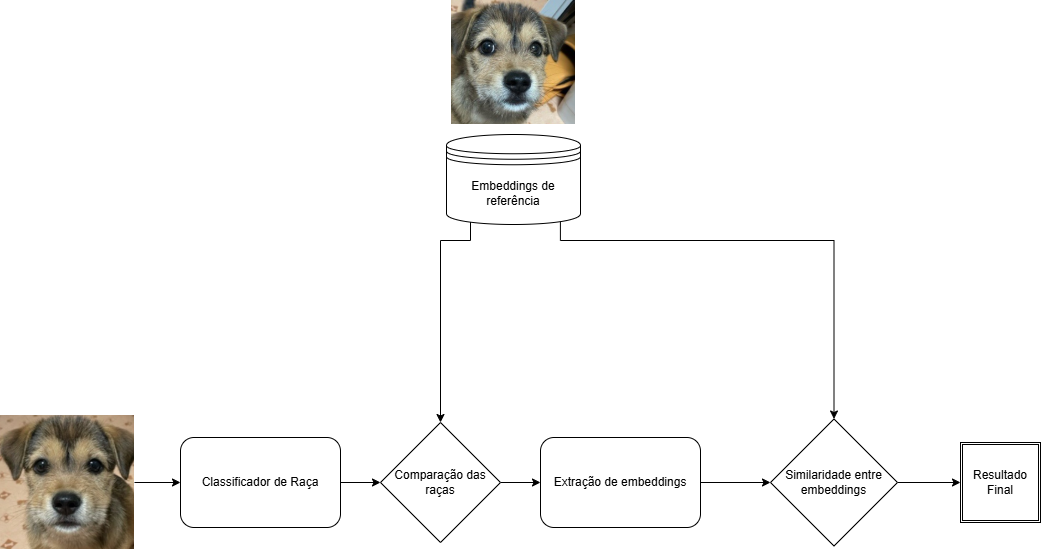
\includegraphics[width=\linewidth]{pipeline_veripet.png}
    \caption{Conceptual VeriPet pipeline. Breed classification and biometric verification are evaluated as separate modules, and breed compatibility is tested as a complementary signal for verification.}
    \label{fig:pipeline}
\end{figure}

\subsection{Breed Classification Dataset}

The breed classifier uses the Stanford Dogs Dataset \cite{khosla2012stanforddogs}, which contains 20,580 images from 120 breeds. Each image includes Pascal VOC bounding-box annotations. The bounding boxes were parsed from XML files and expanded by a 10\% margin in each direction before cropping, reducing background influence while preserving the animal region.

The dataset was split with stratification to preserve class proportions: 70\% for training, 15\% for validation, and 15\% for testing. Table~\ref{tab:stanford_split} summarizes the split. The validation set was used for model selection, while final metrics were computed on the held-out test set.

\begin{table}[t]
\centering
\caption{Stanford Dogs split for breed classification.}
\label{tab:stanford_split}
\begin{tabular}{lrr}
\toprule
Subset & Images & Proportion \\
\midrule
Training & 14,406 & 70\% \\
Validation & 3,087 & 15\% \\
Test & 3,087 & 15\% \\
\midrule
Total & 20,580 & 100\% \\
\bottomrule
\end{tabular}
\end{table}

\subsection{Breed Classification Model}

The classifier uses ConvNeXt-Tiny initialized with ImageNet-1K weights \cite{deng2009imagenet,liu2022convnext}. The final classification layer was replaced with a 120-unit linear layer. The model has 27.9 million trainable parameters. Training used AdamW, a learning rate of $10^{-4}$, weight decay of $10^{-4}$, cosine annealing, cross-entropy loss, batch size 256, mixed precision, and early stopping with patience of eight epochs. The maximum number of epochs was 50, but the best validation model was selected before final testing.

\begin{table}[t]
\centering
\caption{Breed-classification training configuration.}
\label{tab:classification_hparams}
\begin{tabular}{ll}
\toprule
Parameter & Value \\
\midrule
Backbone & ConvNeXt-Tiny \\
Pretraining & ImageNet-1K \\
Optimizer & AdamW \\
Learning rate & $1 \times 10^{-4}$ \\
Weight decay & $1 \times 10^{-4}$ \\
Scheduler & Cosine annealing \\
Loss & Cross-entropy \\
Maximum epochs & 50 \\
Early stopping & 8 epochs patience \\
Batch size & 256 \\
Mixed precision & Enabled \\
\bottomrule
\end{tabular}
\end{table}

The use of bounding-box crops and stratified splits was intended to reduce two common confounders in fine-grained recognition. First, background context should not dominate breed prediction. Second, because Stanford Dogs has unequal class counts, random non-stratified splitting could produce unstable per-breed evaluation for classes with fewer test samples. The final protocol therefore evaluates the classifier under a controlled but still visually diverse setting.

\subsection{Individual Verification Dataset}

The verification module uses the dog subset of PetFace \cite{shinoda2024petface}. The subset used in this work contains 46,755 identities, 168,348 training images, and 35,366 balanced test verification pairs, with an average of 3.6 training images per identity. The limited number of images per identity makes robust metric learning challenging and reflects a realistic biometric scenario in which many identities have only a few samples.

Two datasets are intentionally used because the annotation requirements differ. Stanford Dogs has curated breed labels and bounding boxes but does not provide individual identity labels. PetFace provides individual identities and verification pairs, but its breed labels are imbalanced and less appropriate as the primary source for a fair 120-class breed classifier.

\begin{table}[t]
\centering
\caption{PetFace Dog statistics used for individual verification.}
\label{tab:petface_stats}
\begin{tabular}{lr}
\toprule
Statistic & Value \\
\midrule
Individual identities & 46,755 \\
Training images & 168,348 \\
Images per identity & min. 2, max. 10, mean 3.6 \\
Test verification pairs & 35,366 \\
Positive/negative ratio & 50\% / 50\% \\
\bottomrule
\end{tabular}
\end{table}

\begin{figure}[t]
    \centering
    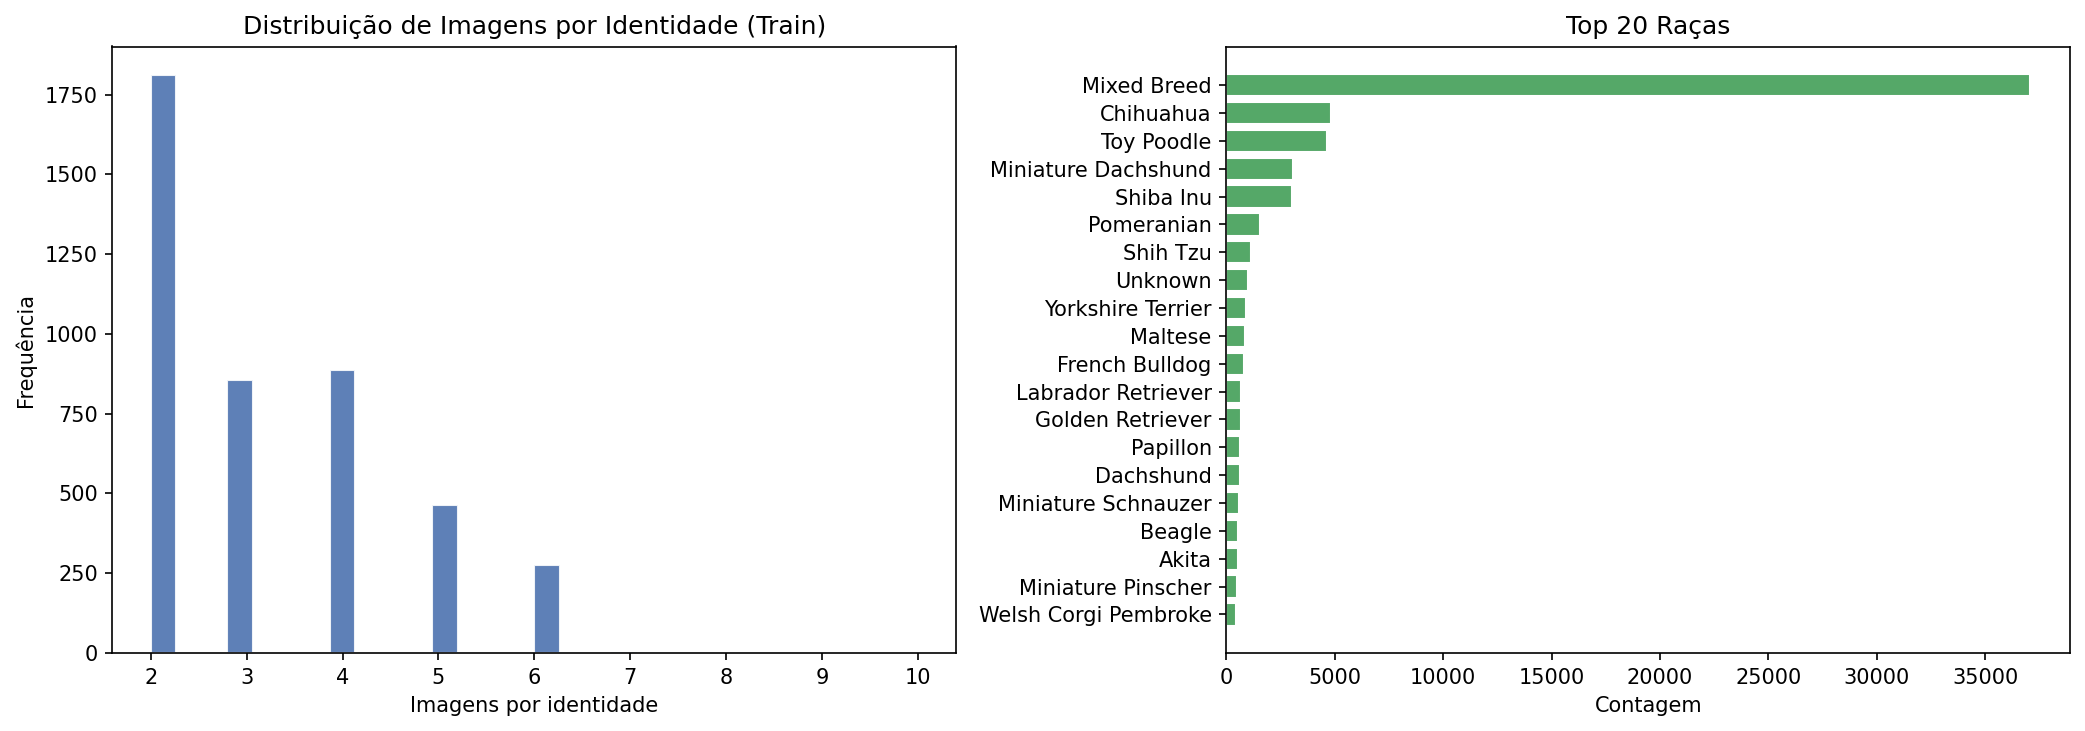
\includegraphics[width=\linewidth]{eda_distributions.png}
    \caption{Exploratory analysis of the PetFace Dog subset. The distribution shows that most identities have few images, while breed metadata is strongly imbalanced.}
    \label{fig:petface_eda}
\end{figure}

\subsection{Verification Model and Decision Rule}

The verifier uses ConvNeXt-Small as the backbone and produces 768-dimensional embeddings. Two training strategies were compared. The first uses standard softmax cross-entropy over training identities, using the penultimate-layer embedding for similarity computation. The second uses ArcFace with margin $m=0.5$ and scale $s=64$, enforcing angular separation among identities \cite{deng2019arcface}.

Both variants used AdamW, learning rate $10^{-4}$, weight decay $10^{-2}$, cosine annealing, 20 epochs, batch size 128, mixed precision, and $224 \times 224$ input resolution. Model selection was based on validation AUC. The decision threshold was calibrated on validation verification pairs and applied unchanged to the test pairs, avoiding test leakage.

\begin{table}[t]
\centering
\caption{Verification training configuration.}
\label{tab:verification_hparams}
\begin{tabular}{ll}
\toprule
Parameter & Value \\
\midrule
Backbone & ConvNeXt-Small \\
Embedding size & 768 \\
Losses & Softmax, ArcFace \\
ArcFace margin & $m=0.5$ \\
ArcFace scale & $s=64$ \\
Optimizer & AdamW \\
Learning rate & $1 \times 10^{-4}$ \\
Weight decay & $1 \times 10^{-2}$ \\
Scheduler & Cosine annealing \\
Epochs & 20 \\
Batch size & 128 \\
Input resolution & $224 \times 224$ \\
\bottomrule
\end{tabular}
\end{table}

For a pair of images $(I_1, I_2)$ with embeddings $e_1$ and $e_2$, the verification score is cosine similarity:
\begin{equation}
    s_{\mathrm{verif}}(I_1,I_2) = \frac{e_1 \cdot e_2}{\|e_1\|\|e_2\|}.
\end{equation}
A pair is accepted as the same individual if $s_{\mathrm{verif}}$ is above the calibrated threshold.

\subsection{Breed-Based Fusion Protocol}

To evaluate whether breed information helps verification, the breed classifier was applied to the verification images. Let $p_c(I)$ be the classifier probability for breed $c$ and image $I$, where $C=120$. Breed compatibility is defined as the probability-distribution overlap:
\begin{equation}
    s_{\mathrm{breed}}(I_1,I_2) = \sum_{c=1}^{C} p_c(I_1)p_c(I_2).
\end{equation}
This score is high when the classifier assigns similar breed distributions to both images. We evaluated a conservative rejection strategy:
\begin{equation}
    s_{\mathrm{fusion}} =
    \begin{cases}
        s_{\mathrm{verif}}, & \text{if } s_{\mathrm{breed}} \geq \tau_{\mathrm{breed}},\\
        0, & \text{otherwise.}
    \end{cases}
\end{equation}
The verifier remains the main decision module, while the classifier can veto pairs with low breed compatibility. As lower baselines, we also evaluated the breed classifier alone as a verifier: a Top-1 agreement rule and a threshold over $s_{\mathrm{breed}}$.

\begin{table}[t]
\centering
\caption{Pair composition in the fusion evaluation set.}
\label{tab:fusion_pairs}
\begin{tabular}{lrr}
\toprule
Pair type & Count & Proportion \\
\midrule
Positive pairs & 18,746 & 50.0\% \\
Hard negatives, same breed & 9,373 & 25.0\% \\
Easy negatives, different breeds & 9,373 & 25.0\% \\
\midrule
Total & 37,492 & 100.0\% \\
\bottomrule
\end{tabular}
\end{table}

\subsection{Experimental Environment}

The experiments were executed in Google Colab with an NVIDIA A100 GPU with 40 GB of memory. Mixed precision was enabled in both classification and verification training to reduce memory use and accelerate training. For the breed classifier, PyTorch 2.x compilation was also enabled. The experimental design separates validation and test usage: validation is used for model selection and threshold calibration, while the test sets are used only for final reporting.

\subsection{Evaluation Metrics}

Breed classification was evaluated with global accuracy, macro precision, macro recall, macro-F1, and weighted-F1. Verification was evaluated with AUC, accuracy, calibrated threshold, and intra-breed accuracy. Intra-breed accuracy is computed on pairs where both dogs belong to the same breed, representing the most difficult scenario because breed-level appearance is shared. The fusion experiment further separates positive pairs, hard negatives (different dogs from the same breed), and easy negatives (different dogs from different breeds).

\section{Experimental Results and Evaluation}

\subsection{Breed Classification Results}

The ConvNeXt-Tiny classifier converged rapidly: the best validation behavior occurred around epoch 7, and early stopping was triggered after epoch 16. Table~\ref{tab:breed_results} reports the final held-out test performance. The model reached 92.55\% global accuracy and 92.4\% macro-F1 across 120 classes, indicating strong generalization for fine-grained breed recognition.

\begin{figure}[t]
    \centering
    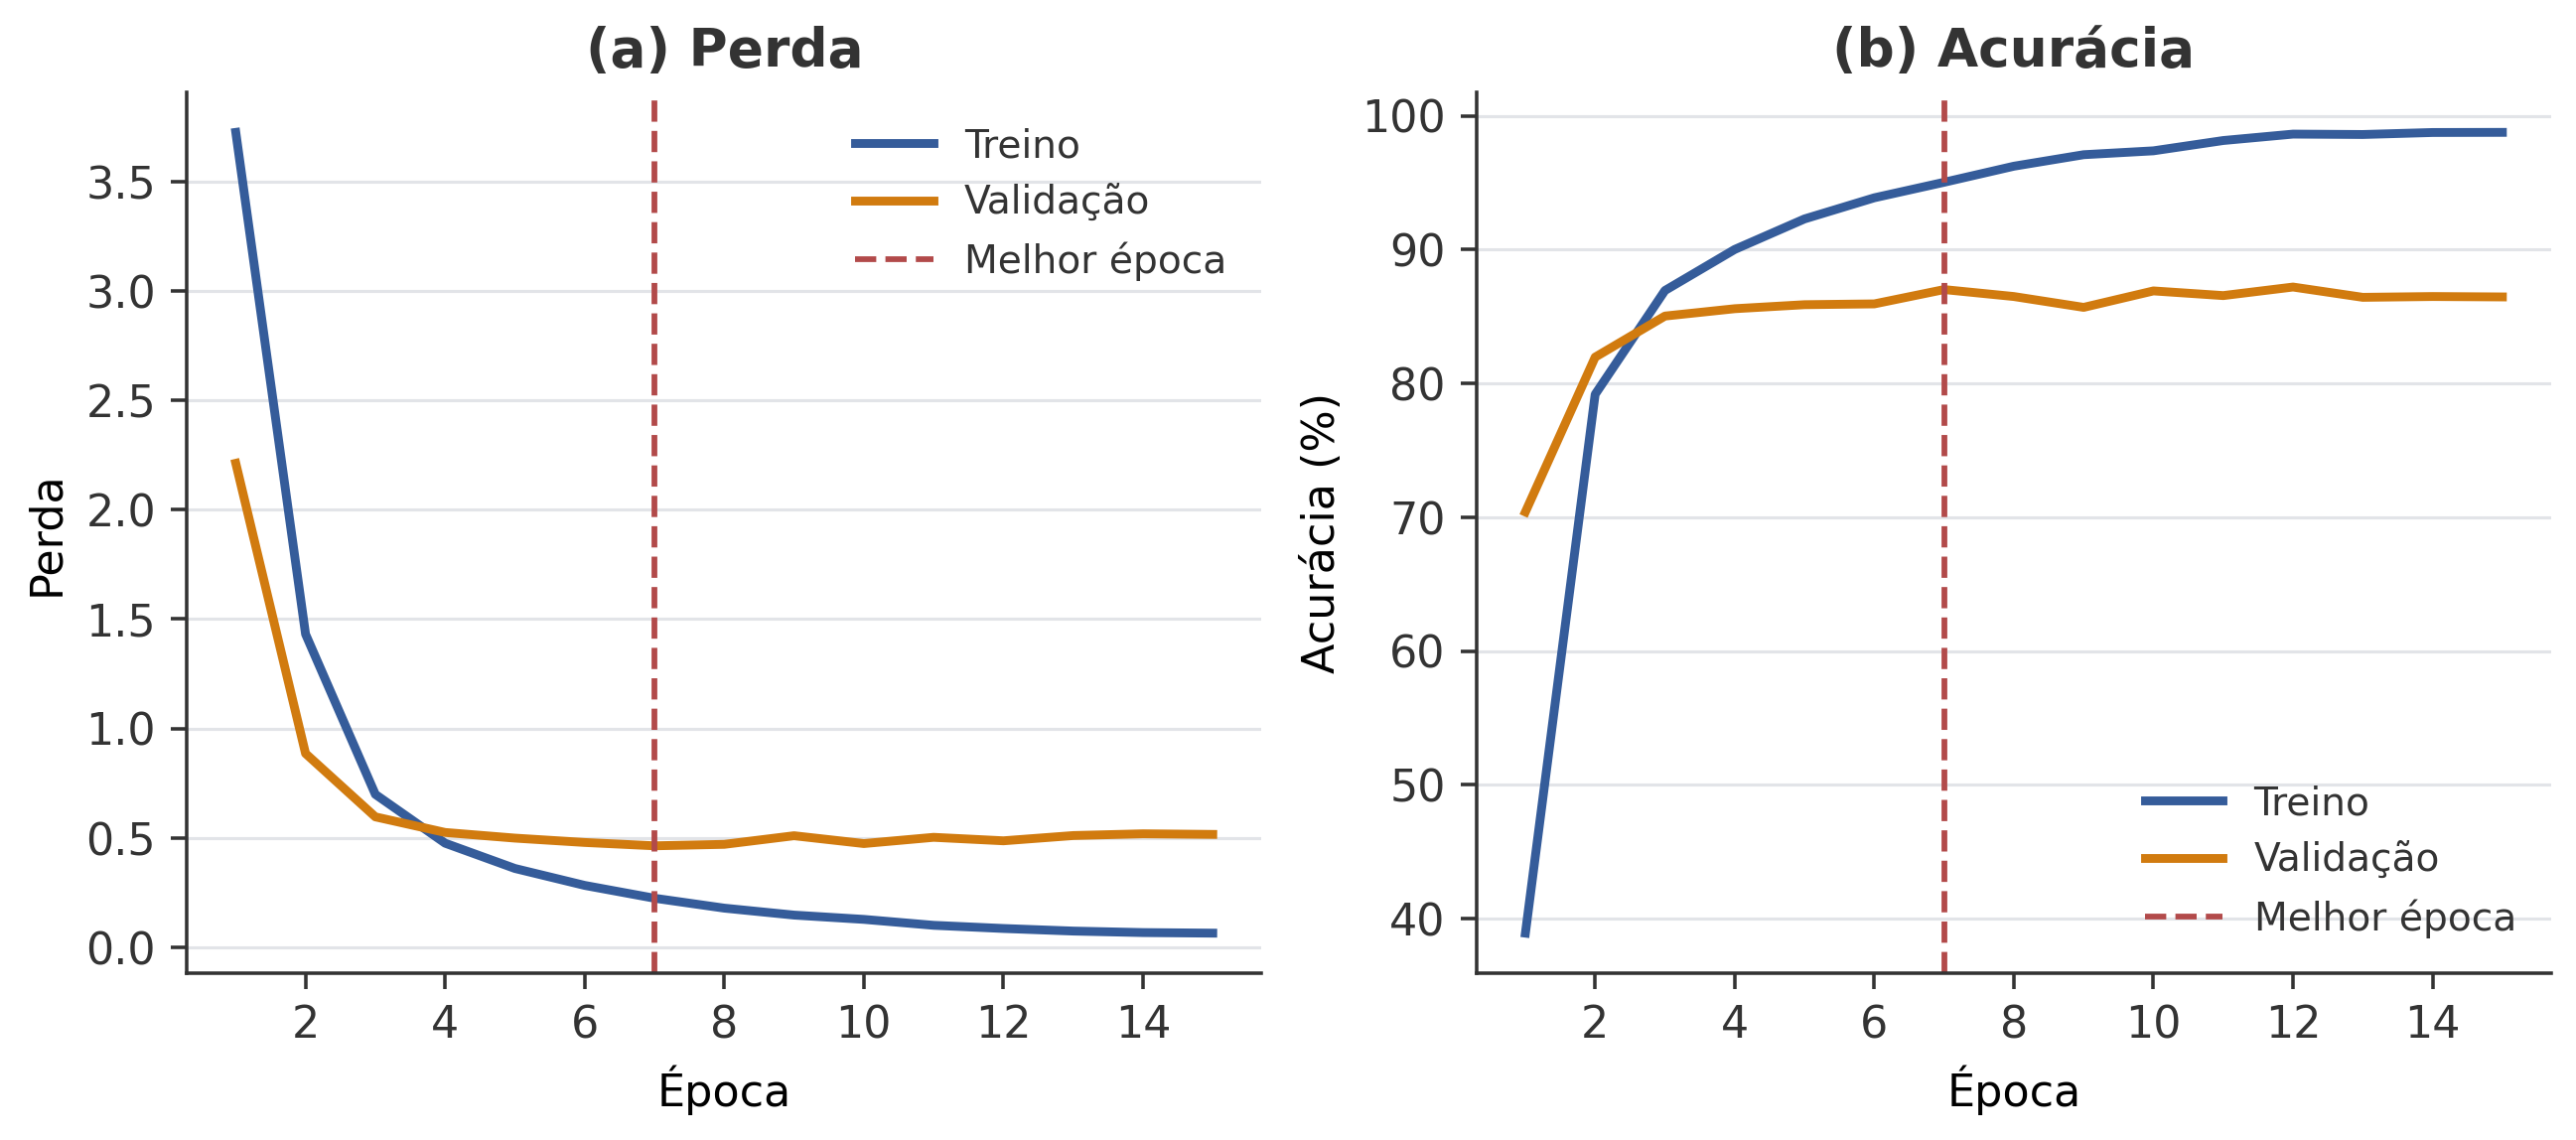
\includegraphics[width=\linewidth]{curvas_treinamento.png}
    \caption{Training curves for the ConvNeXt-Tiny breed classifier. Validation behavior stabilized early, and early stopping prevented unnecessary overfitting.}
    \label{fig:classification_training}
\end{figure}

\begin{table}[t]
\centering
\caption{Breed classification results on the Stanford Dogs test set.}
\label{tab:breed_results}
\begin{tabular}{lr}
\toprule
Metric & Value \\
\midrule
Global accuracy & 92.55\% \\
Macro precision & 92.8\% \\
Macro recall & 92.5\% \\
Macro-F1 & 92.4\% \\
Weighted-F1 & 92.6\% \\
\bottomrule
\end{tabular}
\end{table}

\begin{figure}[t]
    \centering
    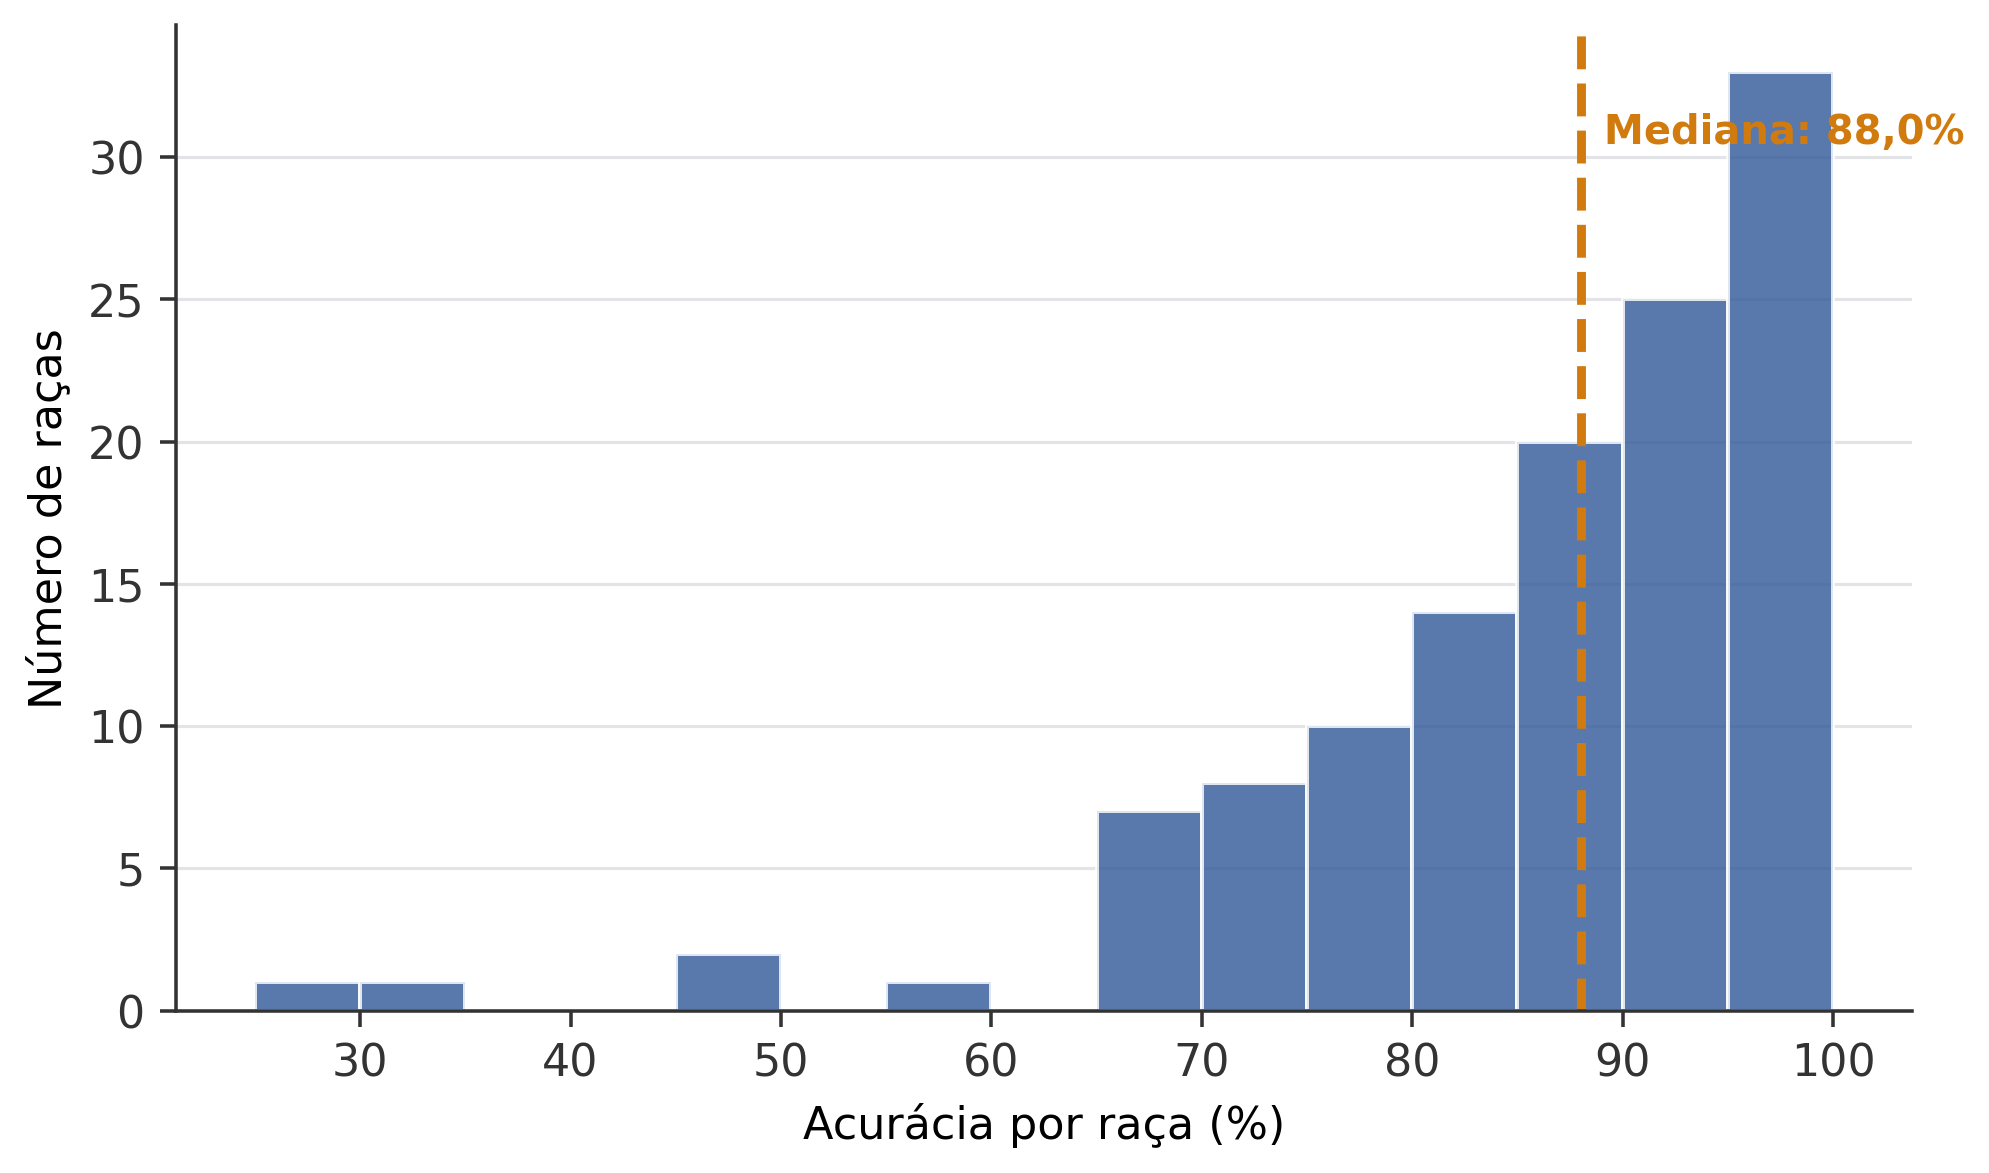
\includegraphics[width=\linewidth]{distribuicao_acuracias.png}
    \caption{Distribution of per-breed accuracies on the Stanford Dogs test set. Most breeds achieved accuracy above 85\%, while errors concentrated in visually similar breed groups.}
    \label{fig:breed_distribution}
\end{figure}

Fig.~\ref{fig:breed_distribution} shows the distribution of per-breed accuracies. Several classes reached 100\% test accuracy, including visually distinctive breeds such as pug, chow, redbone, Doberman, komondor, and soft-coated wheaten terrier. The main failures were concentrated in pairs or families of visually similar breeds. Table~\ref{tab:breed_errors} lists the ten lowest-accuracy breeds and their dominant confusions.

\begin{table*}[t]
\centering
\caption{Lowest-accuracy breeds and dominant confusions in the Stanford Dogs test set.}
\label{tab:breed_errors}
\begin{tabular}{lrrrl}
\toprule
True breed & Support & Errors & Accuracy & Main confusion \\
\midrule
wire-haired fox terrier & 24 & 8 & 66.7\% & Lakeland terrier \\
Border collie & 22 & 7 & 68.2\% & collie \\
Eskimo dog & 22 & 6 & 72.7\% & Siberian husky \\
Staffordshire bullterrier & 23 & 6 & 73.9\% & American Staffordshire terrier \\
miniature poodle & 23 & 6 & 73.9\% & toy poodle \\
standard schnauzer & 23 & 6 & 73.9\% & miniature schnauzer \\
Cardigan & 23 & 5 & 78.3\% & Pembroke \\
collie & 23 & 5 & 78.3\% & Border collie \\
English setter & 24 & 5 & 79.2\% & borzoi \\
Siberian husky & 29 & 6 & 79.3\% & Eskimo dog \\
\bottomrule
\end{tabular}
\end{table*}

The error profile reveals three dominant patterns. First, bidirectional confusions occur between close visual pairs, such as Eskimo dog and Siberian husky or Border collie and collie. Second, size variants are difficult when no external scale reference is available, as seen for poodles and schnauzers. Third, breeds from the same functional or genetic group, such as terriers and Staffordshire-type dogs, share visual traits that make single-image classification ambiguous.

\begin{figure}[t]
    \centering
    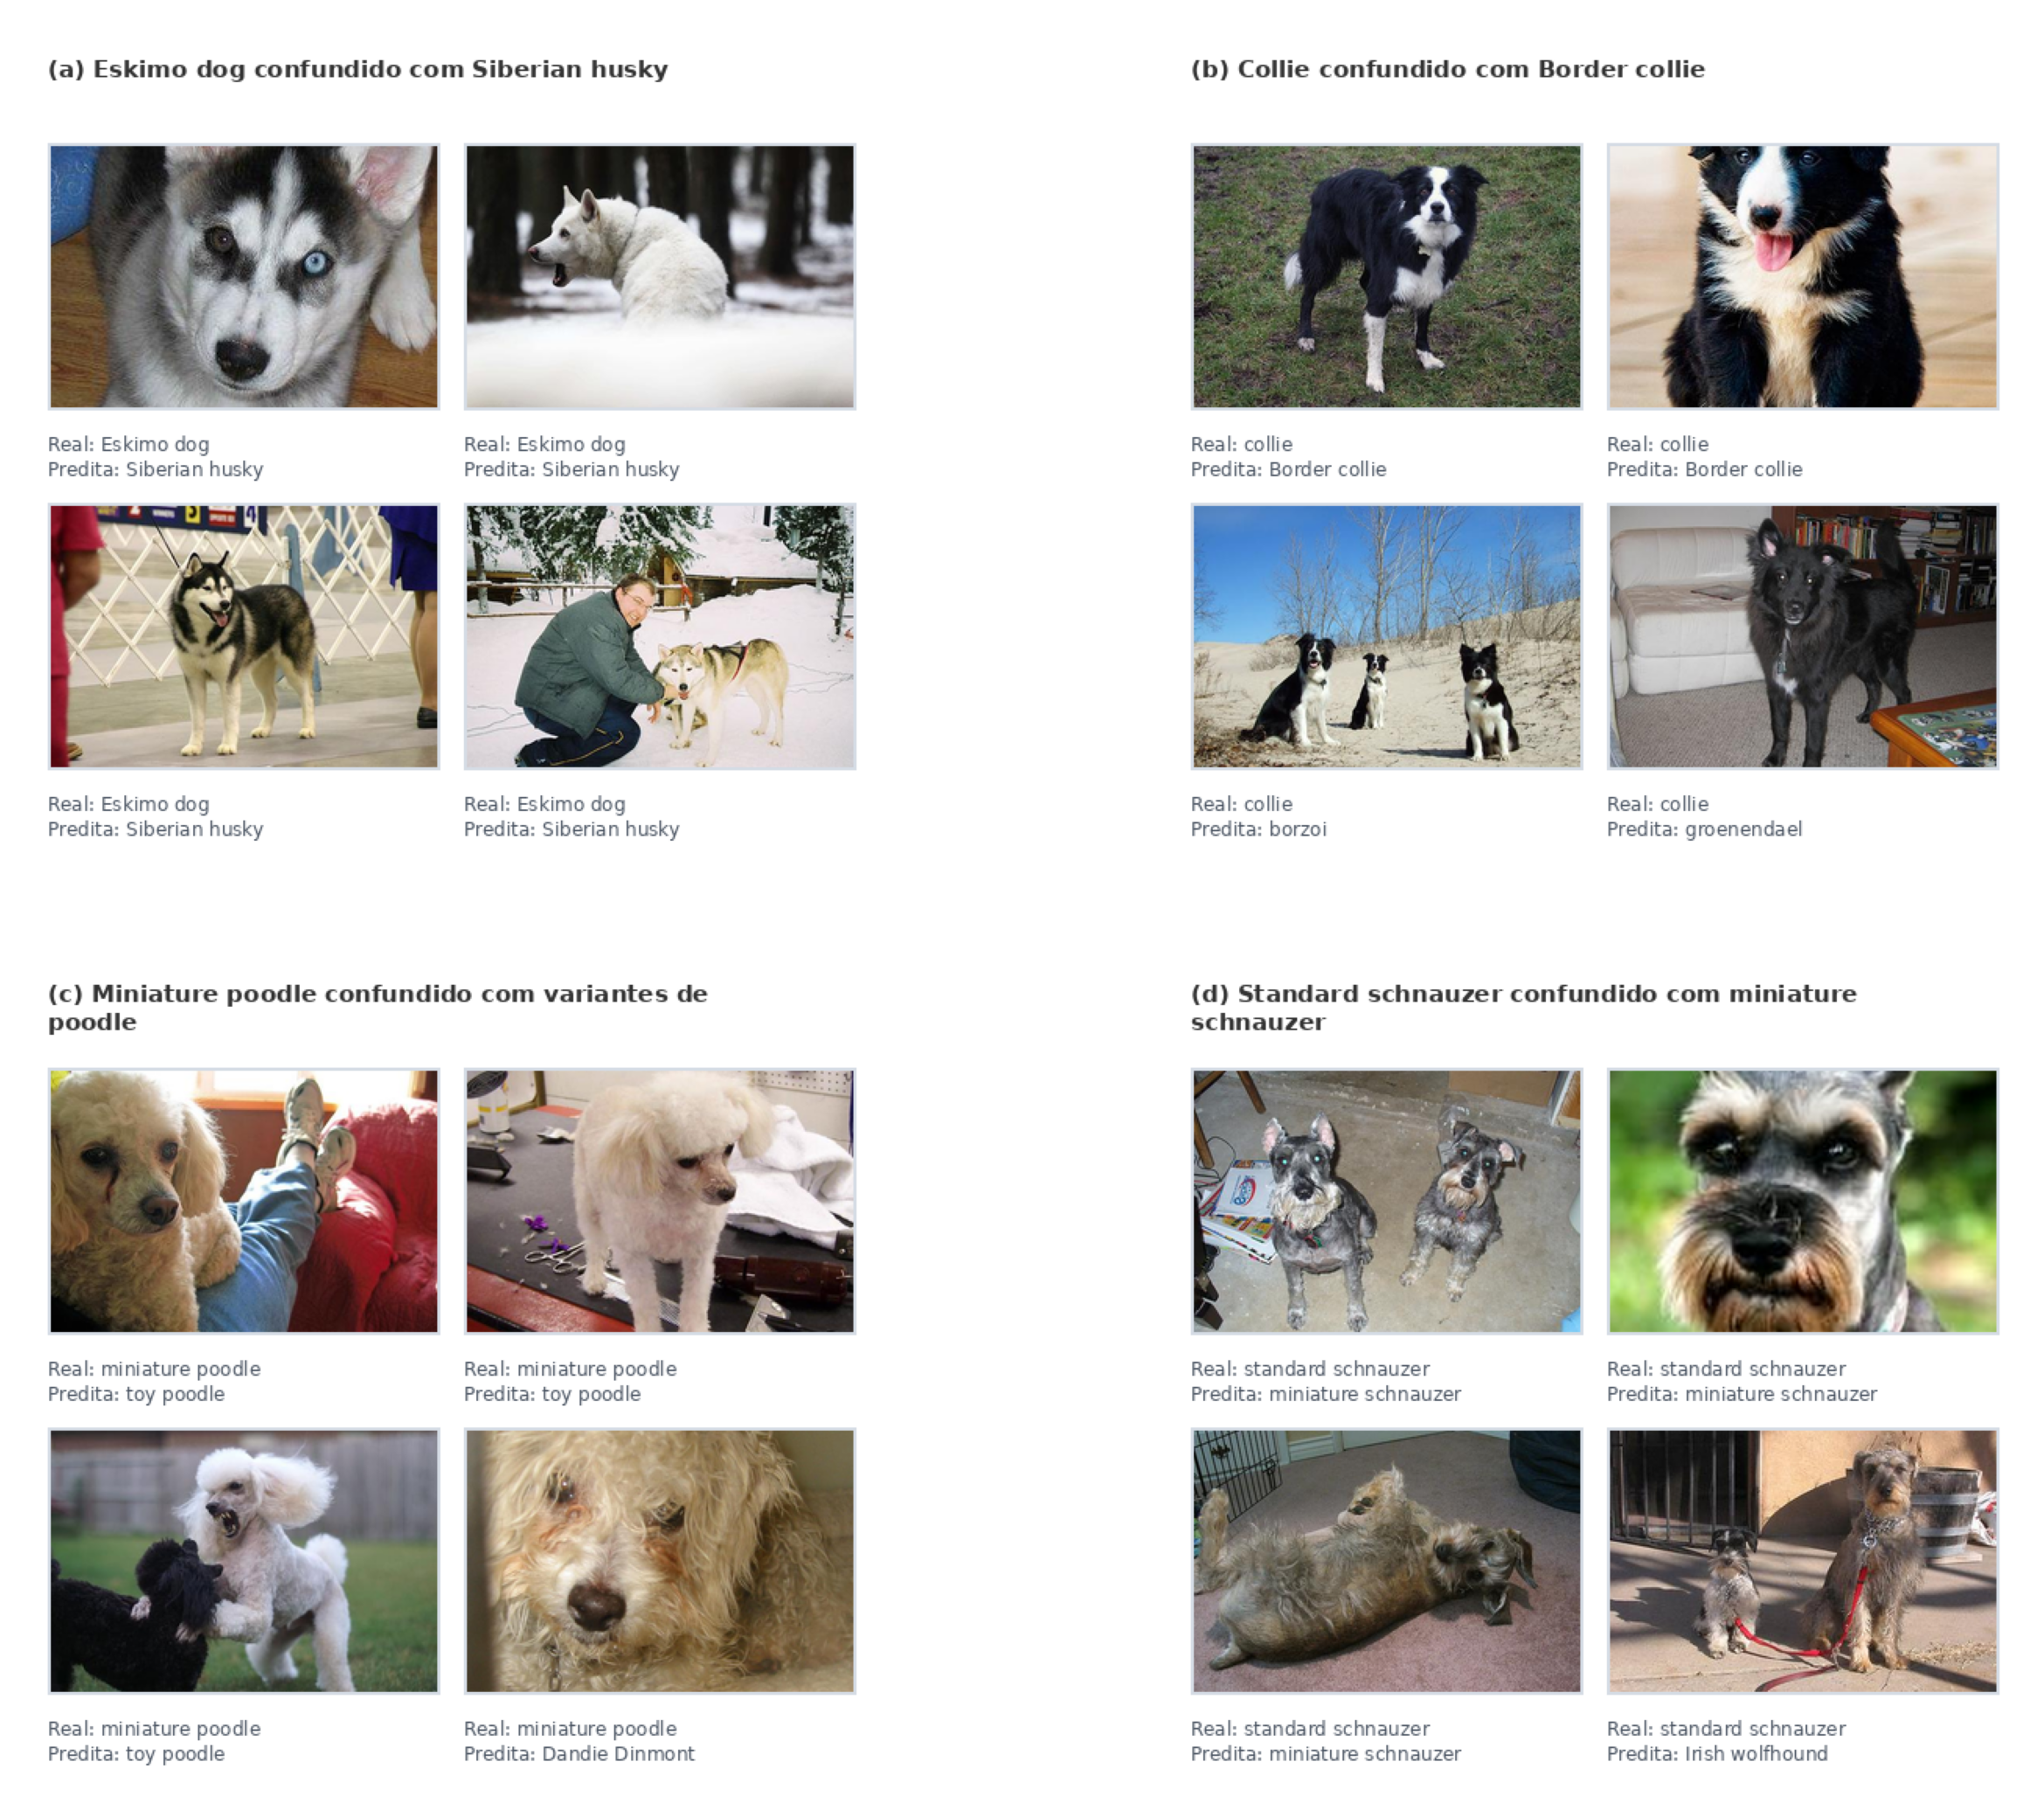
\includegraphics[width=\linewidth]{mosaicos_erros_2x2.png}
    \caption{Examples of misclassified images for visually similar breeds. These errors illustrate the fine-grained nature of dog breed classification.}
    \label{fig:error_mosaic}
\end{figure}

\subsection{Individual Verification Results}

Table~\ref{tab:verification_results} compares ConvNeXt-Small trained with softmax and ArcFace. ArcFace improved every metric. AUC increased from 95.49\% to 97.40\%, global accuracy increased from 86.31\% to 92.52\%, and intra-breed accuracy increased from 80.81\% to 87.88\%. This confirms that angular-margin supervision produces more discriminative identity embeddings for canine verification.

\begin{table}[t]
\centering
\caption{Individual verification results on PetFace Dog test pairs.}
\label{tab:verification_results}
\begin{tabular}{lrrrr}
\toprule
Method & AUC & Acc. & Intra-breed Acc. & Thr. \\
\midrule
Softmax & 95.49\% & 86.31\% & 80.81\% & 0.522 \\
ArcFace & 97.40\% & 92.52\% & 87.88\% & 0.224 \\
\bottomrule
\end{tabular}
\end{table}

\begin{figure}[t]
    \centering
    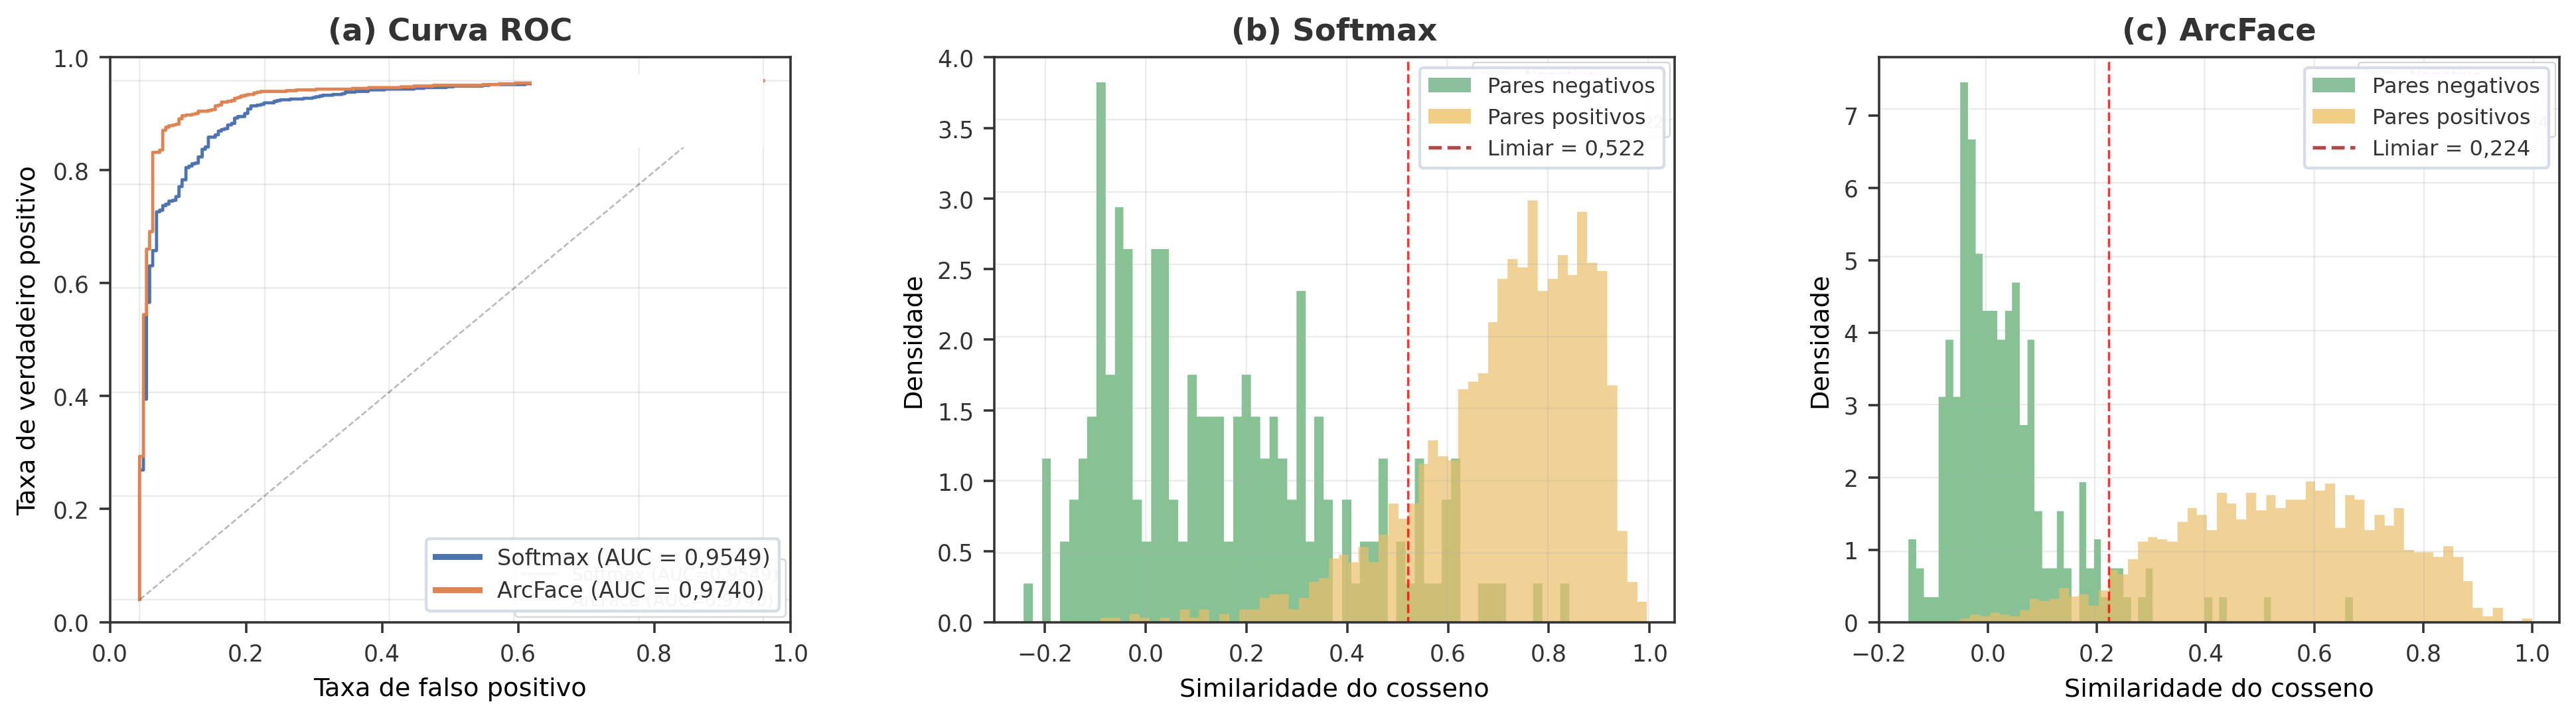
\includegraphics[width=\linewidth]{results_comparison.png}
    \caption{ROC curves and cosine-similarity distributions for softmax and ArcFace verification models. The dashed line marks the validation-calibrated threshold.}
    \label{fig:verification_curves}
\end{figure}

Fig.~\ref{fig:verification_curves} shows that ArcFace yields cleaner score separation between positive and negative pairs. The gap between global accuracy and intra-breed accuracy remains important: even with ArcFace, performance drops by 4.64 percentage points in the intra-breed scenario. This confirms that the main residual challenge is not broad visual separation but distinguishing individuals that share breed-level appearance.

\begin{figure}[t]
    \centering
    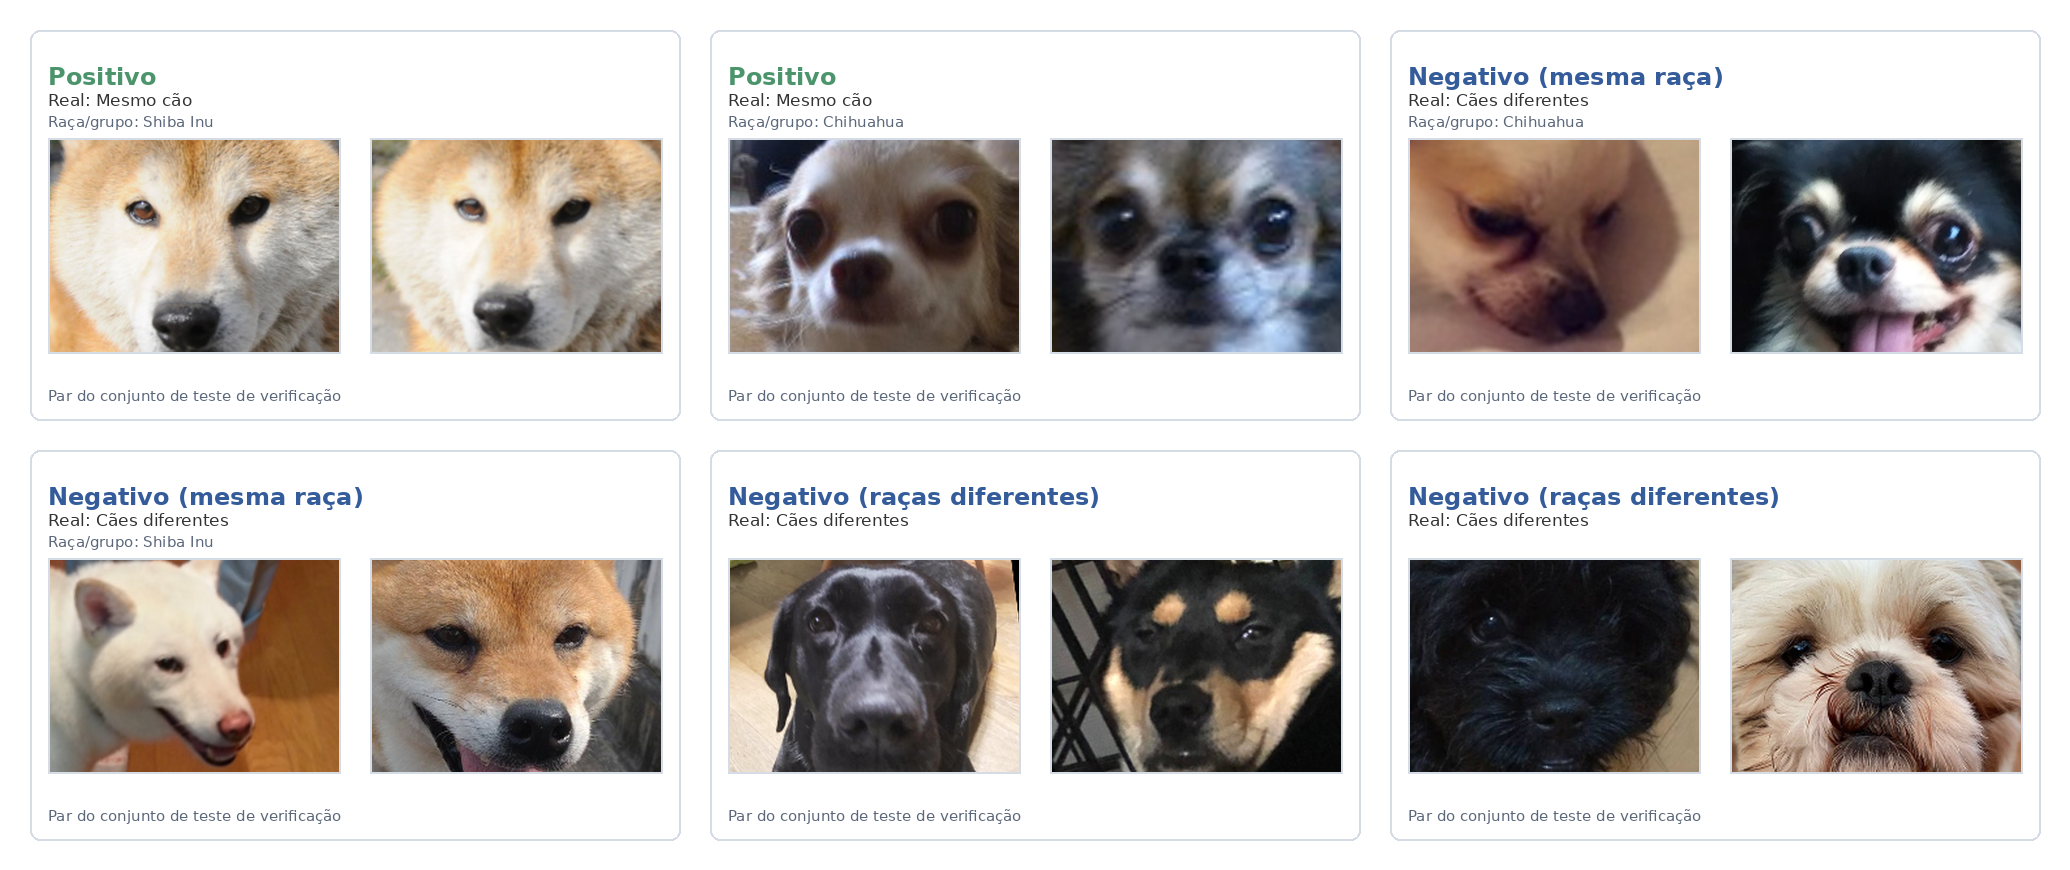
\includegraphics[width=\linewidth]{prediction_examples_results.png}
    \caption{Qualitative examples of ArcFace verification decisions. Each pair is evaluated by cosine similarity and compared with the validation-calibrated threshold.}
    \label{fig:verification_examples}
\end{figure}

\subsection{Breed Classifier as a Verification Filter}

The fusion experiment used 37,492 PetFace verification pairs: 18,746 positives, 9,373 hard negatives, and 9,373 easy negatives. Table~\ref{tab:fusion_results} compares the ArcFace verifier with two breed-only strategies. The Top-1 breed agreement rule performs poorly overall because it rejects many true positive pairs: positive accuracy is only 56.34\%. This means that breed predictions are not stable enough to serve as a strict identity criterion.

\begin{table*}[t]
\centering
\caption{Verification behavior when using the ArcFace verifier and breed classifier-based filters.}
\label{tab:fusion_results}
\begin{tabular}{lrrrr}
\toprule
Method & Overall Acc. & Positives & Hard negatives & Easy negatives \\
\midrule
ArcFace verifier & 93.33\% & 92.80\% & 88.23\% & 99.49\% \\
Breed classifier Top-1 & 76.23\% & 56.34\% & 92.40\% & 99.83\% \\
Breed classifier overlap & 93.10\% & 92.22\% & 88.37\% & 99.59\% \\
\bottomrule
\end{tabular}
\end{table*}

The breed-overlap strategy is much closer to the verifier, reaching 93.10\% overall accuracy. However, it still does not surpass the ArcFace verifier in the global metric and provides no clear gain in the most relevant trade-off. The overlap method slightly improves hard-negative and easy-negative rejection but reduces positive-pair accuracy. In a practical biometric system, false rejection of true matches is costly, especially when images differ in pose, illumination, or framing.

These results indicate that the verifier already learns part of the visual evidence that the breed classifier would provide. The domain mismatch between Stanford Dogs and PetFace also limits fusion: the breed classifier is trained on images that often contain broader body cues, while PetFace verification frequently emphasizes the face. Consequently, breed compatibility is useful for interpretation and possible retrieval constraints but is not robust enough to replace or strongly veto a domain-trained identity verifier.

\section{Scientific Implications}

The experiments support three scientific conclusions. First, modern convolutional models are effective for dog breed recognition, but their errors reveal the limits of category-level supervision in fine-grained animal domains. Second, identity verification benefits strongly from metric-learning objectives: ArcFace produces a substantially better embedding space than softmax for dog identities. Third, breed information and identity information are not interchangeable. Breed labels explain some visual structure, but individual biometrics require representations trained directly for identity discrimination.

For animal biometrics, this suggests that future systems should treat breed as contextual metadata rather than as the primary biometric signal. Breed predictions may help narrow search spaces, explain errors, or organize candidate retrieval, but final verification should rely on identity embeddings calibrated for the target domain. The explicit evaluation of intra-breed pairs is also essential; without it, verification performance may be inflated by easy inter-breed negatives.

\section{Limitations and Threats to Validity}

The study has four main limitations. First, the breed and verification tasks rely on different datasets because the required annotations are different. This is methodologically justified, but it introduces domain shift when breed predictions are reused over PetFace images. Second, PetFace provides many identities but relatively few images per identity; this limits the observed range of age, pose, and long-term appearance variation for each dog. Third, the experiments evaluate image-based verification, not a complete deployed system. Operational components such as image acquisition guidance, quality assessment, duplicate detection, database indexing, privacy policy, and human-in-the-loop review were outside the scope of this paper. Fourth, breed labels are not a perfect biological or visual partition, especially for mixed-breed dogs or visually ambiguous individuals.

These limitations do not invalidate the central comparison between softmax and ArcFace under the same protocol, nor the conclusion that breed-only filtering is insufficient as a primary biometric decision rule. They do, however, define the next research steps. A stronger deployment-oriented benchmark should include longitudinal images, acquisition-quality labels, mixed-breed annotations, and an evaluation protocol that measures false accept and false reject rates at application-specific operating points.

\section{Reproducibility}

The project repository is available at \url{https://github.com/mdrapha/veripet.git}. The reproducibility structure separates application code from research workflows. The reusable experimental code is organized under \texttt{src/veripet/research}, including dataset contracts, model factories, losses, metrics, pair mining, evaluation, plotting, and I/O utilities. The Colab workflows are organized under \texttt{notebooks/colab}, including environment setup, dataset audit, classification workflow, verification workflow, threshold calibration, and error analysis. Result artifacts used in this article are stored with the paper material under \texttt{paper/article\_master/TCC\_\_\_RAPHAEL\_DAMASCENO/figures} and copied into the IEEE article package.

To reproduce the reported results, the expected workflow is: (i) prepare the datasets according to the canonical directory structure described in the repository README; (ii) run the classification workflow for Stanford Dogs; (iii) run the PetFace verification workflow with softmax and ArcFace variants; (iv) run the threshold and fusion evaluation notebooks; and (v) regenerate the result tables and figures. Dataset redistribution is not included in the repository and must follow the original dataset licenses and access conditions.

\section{Conclusion}

This paper presented VeriPet, a deep learning-based experimental pipeline for dog breed classification and individual biometric verification. The ConvNeXt-Tiny breed classifier achieved 92.55\% accuracy and 92.4\% macro-F1 on Stanford Dogs, while the ConvNeXt-Small ArcFace verifier achieved 97.40\% AUC, 92.52\% accuracy, and 87.88\% intra-breed accuracy on PetFace Dog. The comparison with softmax showed that angular-margin learning is important for canine identity embeddings. The breed-fusion study showed that breed compatibility can support interpretation but did not produce a robust improvement over the ArcFace verifier.

The main impact of VeriPet is an experimentally grounded separation between category recognition and biometric identity verification in dogs. This separation clarifies the role of breed as auxiliary context and reinforces the need for identity-specific representation learning, intra-breed evaluation, and reproducible public protocols for animal biometrics.

\balance
\bibliographystyle{IEEEtran}
\bibliography{references}

\end{document}
